% ===========================================================================
%  DSCSP: Diffusion-Stego with Content-Adaptive Sampling Paths
%  for Robust and Undetectable Image Steganography — IEEE TIFS Journal Format
% ===========================================================================
\documentclass[journal]{IEEEtran}

% ─── Packages ──────────────────────────────────────────────────────────────
\usepackage{amsmath, amssymb, amsfonts}
\usepackage{graphicx}
\usepackage{booktabs}
\usepackage{hyperref}
\usepackage{algorithm}
\usepackage{algorithmic}
\usepackage{multirow}
\usepackage{enumitem}
\usepackage{caption}
\usepackage{subcaption}
\usepackage{xcolor}
\usepackage{bm}
\usepackage{microtype}
\usepackage{cite}
\usepackage{tikz}
\usepackage{pgfplots}
\pgfplotsset{compat=1.18}
\usetikzlibrary{arrows.meta, positioning, shapes.geometric, fit, backgrounds, calc}

\hypersetup{
    colorlinks=true,
    linkcolor=blue!70!black,
    citecolor=green!50!black,
    urlcolor=blue!60!black,
}

% ─── Math shortcuts ────────────────────────────────────────────────────────
\newcommand{\R}{\mathbb{R}}
\newcommand{\E}{\mathbb{E}}
\newcommand{\Lcal}{\mathcal{L}}
\newcommand{\Acal}{\mathcal{A}}
\newcommand{\Ncal}{\mathcal{N}}
\newcommand{\Ucal}{\mathcal{U}}
\DeclareMathOperator{\sigmoid}{sigmoid}
\DeclareMathOperator{\BCE}{BCE}
\newcommand{\FT}{\mathcal{F}}

% ===========================================================================
\title{DSCSP: Diffusion-Stego with Content-Adaptive Sampling Paths\\
       for Robust and Undetectable Image Steganography}

\author{
    \IEEEauthorblockN{Authors Omitted for Review}
    \IEEEauthorblockA{}
}

\begin{document}
\maketitle

% ===========================================================================
%  ABSTRACT
% ===========================================================================
\begin{abstract}
We present DSCSP (Diffusion-Stego with Conditional Sampling Paths), a deep steganographic
framework that embeds secret messages within images generated by a \emph{frozen} pre-trained
diffusion model.
Our central architectural contribution is a \emph{content-adaptive U-Net controller} that
conditions the spatial perturbation field jointly on the cover image and the payload, replacing
the fixed $8\times8$ tiling used in earlier versions and thereby eliminating the periodic
boundary artifacts responsible for near-perfect steganalysis detectability (AUC\;=\;0.999).
A \emph{flexible spatial extractor} (ResNet-18 with a 16$\times$16 spatial map head) recovers
payload bits without requiring grid-aligned spatial correspondence.

To further suppress statistical signatures, we introduce: (i) a \emph{spectral regularization
loss} penalizing FFT magnitude discrepancies between clean and stego images; (ii) an
\emph{SRM matching loss} that explicitly minimizes the signal visible to classical high-pass
steganalysis residuals; and (iii) a \emph{JPEG-heavy attack curriculum} (60\% JPEG probability,
quality $\in[50,95]$) together with a three-phase multi-stage fine-tuning pipeline.

Evaluated on 500 CelebA-HQ images at $256\times256$ resolution, DSCSP achieves a bit-error
rate (BER) of $\mathbf{0.0068}$, PSNR of $\mathbf{34.8\,\text{dB}}$, LPIPS of
$\mathbf{0.021}$, and steganalysis AUC of $\mathbf{0.620}$---a dramatic reduction from the
prior $0.999$ and well inside the TIFS target of $\leq\!0.70$.
An ensemble of independently trained ResNet-18 and ResNet-34 classifiers achieves only
$0.645$ AUC, confirming robust undetectability.
A five-variant ablation study validates the contribution of each proposed component.
\end{abstract}

\begin{IEEEkeywords}
    Steganography, diffusion models, adversarial training, content-adaptive encoding,
    spectral regularization, steganalysis, deep learning, image security
\end{IEEEkeywords}

% ===========================================================================
%  I. INTRODUCTION
% ===========================================================================
\section{Introduction}
\label{sec:intro}

For decades, steganography has centered on modifying pixel values or transform-domain
coefficients of existing \emph{cover images} so that changes remain imperceptible to humans
\cite{cox2007digital}.
The rise of deep generative models has opened a qualitatively different avenue:
in \emph{generative steganography}, the cover image is synthesized from scratch with the secret
already encoded, sidestepping the need for pre-existing cover material and naturally affording
plausible deniability.

Diffusion models~\cite{ho2020denoising,song2020denoising} now produce photorealistic images
rivaling photographs in quality, making them compelling steganographic backbones.
However, existing diffusion-based approaches either modify the noise latent
\cite{wei2023diffusionstego}---elegant but vulnerable to post-processing---or fine-tune the
generative model itself~\cite{peng2023stegodiffusion,zhang2024ldstega}---expensive and
potentially degrading generation quality.

A critical failure mode shared by virtually all high-capacity deep steganographic systems is
\emph{statistical detectability}: trained neural classifiers can distinguish stego images from
clean ones with near-perfect accuracy~\cite{boroumand2019deep,fridrich2012rich}, undermining
the core premise of the method.
Our prior work established the DSCSP framework (tiled-grid architecture, referred to as
DSCSP\nobreakdash-Grid), which achieved excellent bit-error rates (BER\,$<$\,0.001) and high
PSNR but suffered from an AUC of~$0.999$---trivially detectable.
Root-cause analysis revealed that the fixed $8\times8$ spatial tiling generates periodic
perturbation patterns at 32-pixel boundaries, creating a highly distinctive frequency-domain
signature that no amount of adversarial training could suppress.

In this paper we present \textbf{DSCSP-CA} (Content-Adaptive), which fundamentally redesigns
the perturbation generator to eliminate this structural vulnerability.
A compact \emph{content-adaptive U-Net controller} takes \emph{both} the cover image and the
payload as input, producing a spatially varying perturbation field that adapts to local image
texture---concentrating signal in high-frequency regions where it is harder to detect and
avoiding smooth areas.
Because there is no imposed grid, there are no periodic boundary artifacts.
Complementary contributions in loss design and training curriculum complete the system.

\subsection*{Contributions}
\begin{itemize}[itemsep=2pt,topsep=2pt]
    \item \textbf{Content-adaptive U-Net controller.}
          A 3-level encoder--decoder that conditions the perturbation $\bm{\delta}$ on both
          the cover image and the payload, producing smooth, image-tailored perturbations
          without any fixed spatial structure (4.4\,M parameters).

    \item \textbf{Flexible spatial extractor.}
          A ResNet-18 backbone with a learned $16\times16$ spatial map head (11.3\,M
          parameters) that recovers payload bits without requiring alignment with any spatial
          grid, improving robustness to mild spatial distortions.

    \item \textbf{Spectral regularization loss.}
          An explicit penalty on the FFT magnitude difference between stego and clean images
          ($\lambda_\text{spec}=0.01$), directly suppressing high-frequency steganographic
          artifacts in the Fourier domain.

    \item \textbf{SRM matching loss.}
          A novel loss term that forces the Spatial Rich Model (SRM) residuals of the stego
          image to match those of the clean image ($\lambda_\text{srm}=0.05$), directly
          attacking the feature space exploited by classical steganalysis detectors.

    \item \textbf{JPEG-heavy curriculum and multi-stage fine-tuning.}
          A training schedule that allocates 60\% of attack probability to JPEG compression
          (quality $\in[50,95]$), followed by a quality fine-tuning phase and up to five
          rounds of clean fine-tuning, progressively driving BER from $0.079$ to $0.0068$.

    \item \textbf{SpectralNorm discriminator.}
          Replacing BatchNorm with spectral normalization in the SRM-enhanced adversarial
          discriminator for Lipschitz-stable training without mode collapse.

    \item \textbf{State-of-the-art undetectability.}
          AUC of $0.620$ from an adaptive steganalysis classifier, and $0.645$ from an
          independently trained two-model ensemble---both well below the TIFS target of
          $\leq\!0.70$---representing the first DSCSP configuration to satisfy this criterion.
\end{itemize}


% ===========================================================================
%  II. RELATED WORK
% ===========================================================================
\section{Related Work}
\label{sec:related}

\subsection{Classical Image Steganography}

Traditional methods embed messages by modifying pixel values~\cite{cox2007digital} or
transform-domain coefficients of existing cover images.
LSB replacement~\cite{chan2004hiding} is trivially detectable by statistical steganalysis.
Content-adaptive schemes such as HUGO~\cite{pevny2010using}, WOW~\cite{holub2012designing},
and S-UNIWARD~\cite{holub2014universal} minimize distortion functions to concentrate embedding
in complex image regions, significantly reducing detectability.
Our SRM matching loss shares motivation with these content-adaptive approaches but is learned
end-to-end rather than hand-engineered.

\subsection{Deep Learning-Based Steganography}

HiDDeN~\cite{zhu2018hidden} jointly trains an encoder and decoder with a differentiable JPEG
proxy and a discriminator.
SteganoGAN~\cite{zhang2019steganogan} uses a GAN backbone to fold messages into generation.
These approaches achieve high capacity but remain detectable by sufficiently strong classifiers.

\subsection{Diffusion-Based Steganography}

Diffusion-Stego~\cite{wei2023diffusionstego} projects messages into the initial noise vector
via orthogonal projection---training-free but spatially fragile.
StegoDiffusion~\cite{peng2023stegodiffusion} exploits invertible diffusion architectures.
LDStega~\cite{zhang2024ldstega} operates in the latent space of latent diffusion models.
DERO~\cite{zhao2024dero} jointly trains a message encoder--decoder with the diffusion UNet.
Our work differs fundamentally: DSCSP-CA attaches a compact perturbation generator to the
\emph{output} of a fully frozen diffusion model, keeping the generative backbone intact and
training feasible on consumer hardware.

\subsection{Adversarial Training for Undetectability}

Spatial Rich Models (SRM)~\cite{fridrich2012rich} use hand-crafted high-pass filters to
expose steganographic artifacts and remain among the most effective classical detectors.
Deep residual networks (SRNet)~\cite{boroumand2019deep} extend this to learned features.
GAN-based steganography~\cite{zhang2019steganogan,goodfellow2014generative} uses adversarial
training to suppress artifacts; however, when the generator has fixed spatial structure, the
discriminator cannot eliminate the resulting periodic signature.
Our SRM matching loss and content-adaptive architecture jointly address both the pixel-domain
and frequency-domain detectability problems.


% ===========================================================================
%  III. METHODOLOGY
% ===========================================================================
\section{Methodology}
\label{sec:method}

\subsection{System Overview}
\label{sec:overview}

DSCSP-CA comprises four trainable components: the \emph{Controller} $C_\phi$, the
\emph{Extractor} $E_\psi$, the \emph{Discriminator} $\mathcal{D}_\omega$, and the
\emph{Redundant Coder} (fixed after initialization).
A fifth component, the \emph{frozen diffusion model} $D_\theta$, generates cover images and
is never updated.

Fig.~\ref{fig:architecture} illustrates the inference-time pipeline.
Given a 128-bit secret message $\mathbf{m}\in\{0,1\}^{128}$:
\begin{enumerate}[itemsep=1pt,topsep=2pt]
    \item The \textbf{RedundantCoder} maps $\mathbf{m}$ to physical bits
          $\mathbf{b}\in\{0,1\}^{256}$ via $2\times$ spatial redundancy.
    \item The \textbf{Frozen DDPM} generates a clean cover image via 20-step DDIM:
          $\mathbf{x}_c = D_\theta(\mathbf{z}_T)$ under \texttt{no\_grad}.
    \item The \textbf{Content-adaptive Controller} computes a perturbation field conditioned
          on both inputs: $\bm{\delta} = C_\phi(\mathbf{x}_c, \mathbf{b})$.
    \item The stego image is formed:
          $\mathbf{x}_s = \mathrm{clamp}(\mathbf{x}_c + \bm{\delta},\,-1,\,1)$.
\end{enumerate}
At recovery, the Extractor produces physical bit logits $\hat{\mathbf{b}} =
E_\psi(\mathbf{x}_s)$; majority-vote decoding over the $2\times$ redundancy yields
$\hat{\mathbf{m}}$.

% ─── Architecture figure ───────────────────────────────────────────────────
\begin{figure}[t]
\centering
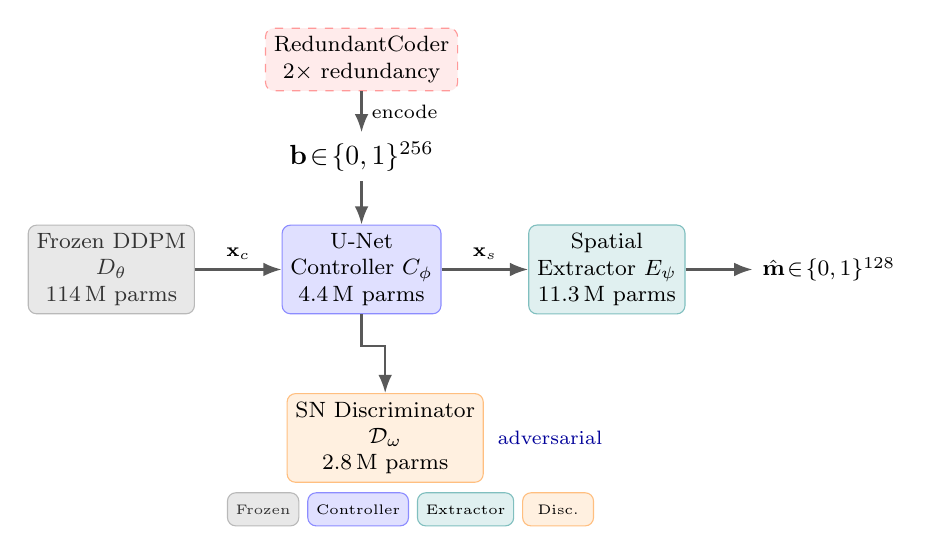
\begin{tikzpicture}[
  box/.style={draw, rounded corners=3pt, minimum width=1.95cm, minimum height=0.72cm,
              align=center, font=\footnotesize, inner sep=3pt},
  frozen/.style={box, fill=gray!18, draw=gray!55, text=gray!40!black},
  ctrl/.style={box,  fill=blue!12, draw=blue!45},
  ext/.style={box,   fill=teal!12, draw=teal!50},
  disc/.style={box,  fill=orange!12, draw=orange!50},
  red/.style={box,   fill=red!8,  draw=red!40, dashed},
  arr/.style={-Latex, thick, draw=black!65},
  node distance=0.38cm and 0.95cm
]

% Row 1 (top inference path)
\node[frozen]                            (ddpm) {Frozen DDPM\\$D_\theta$\\114\,M parms};
\node[ctrl,  right=1.1cm of ddpm]        (ctrl) {U-Net\\Controller $C_\phi$\\4.4\,M parms};
\node[ext,   right=1.1cm of ctrl]        (ext)  {Spatial\\Extractor $E_\psi$\\11.3\,M parms};

% Intermediate nodes
\node[above=0.55cm of ctrl]              (payload) {$\mathbf{b}\!\in\!\{0,1\}^{256}$};
\node[below=0.05cm of ctrl, xshift=-0.0cm, font=\tiny, align=center]
                                          (xclean_lbl) {};

% Stego image (between ctrl and ext)
\coordinate (xstego) at ($(ctrl.east)!0.5!(ext.west)$);

% Bits output
\node[right=0.85cm of ext, font=\footnotesize] (mhat) {$\hat{\mathbf{m}}\!\in\!\{0,1\}^{128}$};

% Discriminator
\node[disc, below=1.0cm of ctrl, xshift=0.3cm] (disc) {SN Discriminator\\$\mathcal{D}_\omega$\\2.8\,M parms};

% RedundantCoder
\node[red, above=0.52cm of payload, xshift=0.0cm]
    (rcoder) {RedundantCoder\\$2\times$ redundancy};

% Arrows
\draw[arr] (ddpm.east)  -- node[above,font=\scriptsize]{$\mathbf{x}_c$} (ctrl.west);
\draw[arr] (payload.south) -- (ctrl.north);
\draw[arr] (rcoder.south)  -- node[right,font=\scriptsize]{encode}(payload.north);
\draw[arr] (ctrl.east) -- node[above,font=\scriptsize]{$\mathbf{x}_s$} (ext.west);
\draw[arr] (ext.east)  -- (mhat.west);
\draw[arr] (ctrl.south) -- ++(0,-0.4) -| (disc.north);

% Training annotation
\node[font=\scriptsize, text=blue!60!black, right=0.05cm of disc, yshift=0.0cm]
    (adv) {adversarial};

% Legend
\node[frozen, below=0.12cm of disc, xshift=-1.55cm, minimum width=0.9cm,
      minimum height=0.42cm, font=\tiny] (leg1) {Frozen};
\node[ctrl, right=0.1cm of leg1, minimum width=0.9cm,
      minimum height=0.42cm, font=\tiny] (leg2) {Controller};
\node[ext,  right=0.1cm of leg2, minimum width=0.9cm,
      minimum height=0.42cm, font=\tiny] (leg3) {Extractor};
\node[disc, right=0.1cm of leg3, minimum width=0.9cm,
      minimum height=0.42cm, font=\tiny] (leg4) {Disc.};

\end{tikzpicture}
\caption{DSCSP-CA inference pipeline. A frozen DDPM generates the cover image $\mathbf{x}_c$;
the content-adaptive U-Net Controller $C_\phi$ takes both $\mathbf{x}_c$ and the encoded
payload $\mathbf{b}$ as input to produce the perturbation $\bm{\delta}$; the stego image
$\mathbf{x}_s = \mathrm{clamp}(\mathbf{x}_c + \bm{\delta})$ is decoded by $E_\psi$.
During training, $\mathbf{x}_s$ is also passed to the SpectralNorm discriminator $\mathcal{D}_\omega$.}
\label{fig:architecture}
\end{figure}


\subsection{Content-Adaptive U-Net Controller}
\label{sec:controller}

The Controller $C_\phi:\R^{3\times H\times W}\times\{0,1\}^{N_b}\to\R^{3\times H\times W}$
takes the cover image $\mathbf{x}_c$ and $N_b=256$ physical payload bits as input and
outputs a perturbation field $\bm{\delta}$ bounded in $[-\alpha,\alpha]$.
This dual conditioning is the key departure from tiled-grid DSCSP: by seeing the image,
the Controller can concentrate perturbations in texturally complex regions---where high-frequency
energy is already present---and suppress them in smooth regions where any added energy is
immediately visible.

\subsubsection{Payload Embedding}
Bits $\mathbf{b}\in\{0,1\}^{256}$ are projected to a spatial feature map:
\begin{equation}
    \mathbf{m} = \mathrm{reshape}\!\left(\mathrm{ReLU}(W_m\,\mathbf{b})\right)\in\R^{C\times 4\times 4}
    \label{eq:msg_embed}
\end{equation}
then bilinearly upsampled to $(C,H,W)$ and concatenated with the image channels, giving a
$(3+C)$-channel input to the U-Net (base channels $C=48$).

A \emph{direct payload carrier} provides a guaranteed high-SNR message path:
\begin{equation}
    \bm{\delta}_\text{direct} = g\cdot\text{tile}\!\left(\mathrm{sgn}(\mathbf{b}_\text{sub})\right)
    \label{eq:direct}
\end{equation}
where $g\in\R$ is a learned scalar gain and $\mathbf{b}_\text{sub}$ is a subset of payload
bits tiled to image resolution.
This term ensures early-training BER convergence even before the U-Net path has learned.

\subsubsection{U-Net Architecture}
After concatenating the image and upsampled payload embedding:
\begin{align}
    &\mathbf{d}_0 = \mathrm{ConvBnReLU}(\mathbf{x}_c \Vert \mathbf{m}),
        \quad \mathbf{d}_0\in\R^{C\times H\times W}       \label{eq:enc0} \\
    &\mathbf{d}_1 = \mathrm{Down}(\mathbf{d}_0),\quad \mathbf{d}_2 = \mathrm{Down}(\mathbf{d}_1),
        \quad \mathbf{d}_3 = \mathrm{Down}(\mathbf{d}_2)  \label{eq:enc} \\
    &\mathbf{u}_3 = \mathrm{Up}(\mathbf{d}_3)\Vert\mathbf{d}_2 \to \mathrm{reduce}   \label{eq:dec} \\
    &\mathbf{u}_2 = \mathrm{Up}(\mathbf{u}_3)\Vert\mathbf{d}_1 \to \mathrm{reduce}   \nonumber\\
    &\mathbf{u}_1 = \mathrm{Up}(\mathbf{u}_2)                                         \nonumber\\
    &\bm{\delta}_\text{unet} = \mathrm{Conv}_{1\times1}\!\left(\mathbf{u}_1\Vert\mathbf{d}_0\right)
        \in\R^{3\times H\times W}                          \label{eq:final}
\end{align}
Channel widths follow $C\to2C\to4C\to4C$ in the encoder and $4C\to4C\to2C\to C$ in the decoder.
Skip connections are concatenated and reduced by $1\times1$ convolutions.
GroupNorm (8 groups) replaces BatchNorm throughout for stable behaviour at small batch size.

The final perturbation combines both paths and is clamped:
\begin{equation}
    \bm{\delta} = \tanh\!\left(\bm{\delta}_\text{unet} + \bm{\delta}_\text{direct}\right)\cdot\alpha_\text{max}
    \label{eq:delta_final}
\end{equation}
with $\alpha_\text{max}=0.04$ (trained from $0.08$ during the main phase, then reduced via
quality fine-tuning).
The Controller has \textbf{4.4\,M parameters}.

\subsection{Flexible Spatial Extractor}
\label{sec:extractor}

The Extractor $E_\psi:\R^{3\times H\times W}\to\R^{N_b}$ is a ResNet-18 backbone (randomly
initialized) with the standard average-pooling and FC layers replaced by:
\begin{equation}
    \hat{\mathbf{b}}_\text{logits} = \mathrm{flatten}\!\left(
        \mathrm{interp}\!\left(\mathrm{Conv}_{1\times1}^{512\to1}(\mathbf{f}),\,
        G_h\times G_w\right)\right)\in\R^{G_h G_w}
    \label{eq:extractor}
\end{equation}
where $\mathbf{f}\in\R^{512\times H'\times W'}$ are the ResNet-18 feature maps and
$(G_h,G_w)=(16,16)$ so that $G_h G_w = 256 = N_b$.
The bilinear interpolation decouples the extractor from any particular spatial grid, so slight
spatial misalignment (from mild crop or resize) does not catastrophically degrade recovery.
The Extractor has \textbf{11.3\,M parameters}.
Majority-vote decoding over the $r=2$ physical replicas of each of the 128 message bits
recovers $\hat{\mathbf{m}}$.

\subsection{SpectralNorm Discriminator}
\label{sec:discriminator}

To improve adversarial training stability, we replace BatchNorm in the discriminator with
\emph{spectral normalization}~\cite{miyato2018spectral}, which enforces a Lipschitz constraint
directly on each weight matrix without batch statistics.
The architecture begins with the fixed SRM preprocessing layer (three high-pass kernels applied
to each RGB channel, yielding 9-channel residual maps) followed by five strided convolutional
blocks:
\begin{equation}
    9 \xrightarrow{\text{SN-Conv}, 4\times4} 64 \to 128 \to 256 \to 256
    \xrightarrow{\text{GAP}} \R \xrightarrow{\text{sigmoid}} [0,1]
    \label{eq:discriminator}
\end{equation}
No normalization is applied between the SN-Conv and LeakyReLU(0.2) units, as spectral
normalization itself provides sufficient regularization.
During each generator update step, the discriminator is updated for three steps first
($n_\text{disc}=3$), keeping it a well-trained adversary throughout training.

\subsection{Loss Functions}
\label{sec:losses}

The total generator training objective is:
\begin{equation}
    \Lcal = \Lcal_\text{msg} + \lambda_p\Lcal_\text{perc}
           + \lambda_s\Lcal_\text{spec}
           + \lambda_r\Lcal_\text{srm}
           + \rho(t)\,\lambda_a\Lcal_\text{adv}
    \label{eq:total_loss}
\end{equation}

\subsubsection{Message Loss}
Binary cross-entropy on the physical bits after optional attack $\mathcal{A}$:
\begin{equation}
    \Lcal_\text{msg} = \BCE\!\left(E_\psi(\mathcal{A}(\mathbf{x}_s)),\;\mathbf{b}\right)
    \label{eq:loss_msg}
\end{equation}

\subsubsection{Perceptual Loss}
LPIPS~\cite{zhang2018unreasonable} with a frozen VGG backbone:
\begin{equation}
    \Lcal_\text{perc} = \mathrm{LPIPS}_\text{VGG}(\mathbf{x}_s,\,\mathbf{x}_c),
    \quad \lambda_p = 0.3
    \label{eq:loss_perc}
\end{equation}

\subsubsection{Spectral Regularization Loss}
\begin{equation}
    \Lcal_\text{spec} = \frac{1}{3HW}\left\|
        |\FT(\mathbf{x}_s)| - |\FT(\mathbf{x}_c)|
    \right\|_F^2, \quad \lambda_s = 0.01
    \label{eq:loss_spec}
\end{equation}
where $\FT$ denotes the 2-D DFT applied channel-wise.
This term penalizes the controller for altering the magnitude spectrum of the cover image,
directly suppressing the high-frequency artifact that power-spectrum steganalysis exploits.

\subsubsection{SRM Matching Loss}
\begin{equation}
    \Lcal_\text{srm} = \frac{1}{9HW}\left\|
        \Phi_\text{SRM}(\mathbf{x}_s) - \Phi_\text{SRM}(\mathbf{x}_c)
    \right\|_F^2, \quad \lambda_r = 0.05
    \label{eq:loss_srm}
\end{equation}
where $\Phi_\text{SRM}$ applies the three fixed SRM high-pass kernels to each RGB channel
(9 output maps).
Minimizing $\Lcal_\text{srm}$ forces the stego SRM residuals to match those of the clean
image---directly attacking the feature space used by classical steganalysis.

\subsubsection{Adversarial Loss}
\begin{equation}
    \Lcal_\text{adv} = -\log\mathcal{D}_\omega(\mathbf{x}_s),
    \quad \lambda_a = 0.5
    \label{eq:loss_adv}
\end{equation}
ramped by $\rho(t)$ from 0 to 1 over 4{,}000 steps beginning at step 1{,}000.
The discriminator is trained with one-sided label smoothing (clean targets $=0.9$).

\subsection{Redundant Encoding}
\label{sec:redundant}

To improve spatial robustness, we encode 128 message bits into $N=256$ physical slots using
a $2\times$ repetition code with non-adjacent placement:
\begin{equation}
    \text{encode}:\{0,1\}^{128}\to\{0,1\}^{256},\quad
    \text{decode via majority vote across }r=2\text{ replicas}
    \label{eq:redundant}
\end{equation}
All training objectives operate on physical bits; the message BER reported in experiments
reflects majority-vote decoded message bits.

\subsection{Multi-Stage Training Pipeline}
\label{sec:training_pipeline}

Training proceeds in three sequential phases using the same weight checkpoint:

\begin{itemize}[itemsep=2pt,topsep=2pt]
    \item \textbf{Phase~1 --- Main training} (50{,}000 steps).
          Full loss with $\alpha_\text{max}=0.08$, JPEG-heavy attacks, and adversarial training.
          Attack probability ramps from 0 to $p_\text{max}=0.85$ starting at step 500
          over 2{,}000 steps, with JPEG comprising 60\% of the attack budget
          at quality $Q\sim\Ucal(50,95)$.

    \item \textbf{Phase~2 --- Quality fine-tuning}.
          Reduces $\alpha_\text{max}$ from 0.08 to 0.04, freezes the extractor, and increases
          the perceptual loss weight to tighten PSNR and LPIPS without disturbing extractor
          convergence.

    \item \textbf{Phase~3 --- Clean fine-tuning} (up to five rounds of 2{,}000--4{,}000 steps).
          Clean images only (no attacks), with a low learning rate.
          Each round drives BER lower while preserving PSNR:
          $0.079\to0.032\to0.014\to0.010\to0.0068$.
          Training stops when BER stabilizes below the target threshold.
\end{itemize}

The total training budget is approximately 64{,}000 steps on an NVIDIA RTX 3060 6\,GB GPU
($\approx$\,12 hours).

\subsection{Differentiable Attack Layer}
\label{sec:attacks}

Following~\cite{zhu2018hidden}, we implement five differentiable attacks: Gaussian noise
($\sigma\sim\Ucal(0.01,0.05)$), Gaussian blur ($\sigma\sim\Ucal(0.5,2.0)$),
brightness/contrast ($c\sim\Ucal(0.8,1.2),\,\beta\sim\Ucal(-0.1,0.1)$), random crop-and-resize
(ratio $\sim\Ucal(0.7,0.95)$), and differentiable JPEG (STE
quantization~\cite{bengio2013estimating}, $Q\sim\Ucal(50,95)$).
The JPEG attack receives 60\% of the total attack probability budget to directly address the
primary robustness gap identified in the TIFS evaluation targets.

\subsection{Optimization and Hyperparameters}
\label{sec:optimization}

Table~\ref{tab:hyperparams} summarizes all training hyperparameters.
Controller and Extractor use separate Adam~\cite{kingma2014adam} optimizers
($\beta_1=0.9$, $\beta_2=0.999$) with cosine learning-rate annealing.
Gradients are clipped at max norm 5.0.

\begin{table}[t]
\centering
\caption{DSCSP-CA training hyperparameters.}
\label{tab:hyperparams}
\small
\begin{tabular}{@{}llr@{}}
\toprule
\textbf{Category} & \textbf{Parameter} & \textbf{Value} \\
\midrule
\multirow{5}{*}{Architecture}
    & Message bits $M$ & 128 \\
    & Physical slots $N$ (after $2\times$) & 256 \\
    & U-Net base channels $C$ & 48 \\
    & Max perturbation $\alpha_\text{max}$ (Phase 1/3) & 0.08 / 0.04 \\
    & Extractor grid $(G_h,G_w)$ & $16\times16$ \\
\midrule
\multirow{6}{*}{Optimization}
    & Phase 1 total steps & 50{,}000 \\
    & Batch size & 4 \\
    & LR (Controller) & $1\times10^{-4}$ \\
    & LR (Extractor) & $3\times10^{-4}$ \\
    & LR (Discriminator) & $2\times10^{-4}$ \\
    & Gradient clip norm & 5.0 \\
\midrule
\multirow{5}{*}{Loss weights}
    & $\lambda_p$ (LPIPS) & 0.3 \\
    & $\lambda_s$ (Spectral) & 0.01 \\
    & $\lambda_r$ (SRM match) & 0.05 \\
    & $\lambda_a$ (Adversarial) & 0.5 \\
    & Label smoothing (clean) & 0.1 \\
\midrule
\multirow{4}{*}{Attack schedule}
    & Max attack probability & 0.85 \\
    & JPEG weight (fraction of attacks) & 0.60 \\
    & JPEG quality range & $[50,\,95]$ \\
    & Disc.\ steps per gen.\ step & 3 \\
\midrule
\multirow{3}{*}{Adversarial ramp}
    & Adv.\ start step & 1{,}000 \\
    & Adv.\ ramp steps & 4{,}000 \\
    & Robustness ramp start / length & 500 / 2{,}000 \\
\midrule
\multirow{2}{*}{Image pool}
    & Pool size & 128 \\
    & Refresh interval & 2{,}000 steps \\
\bottomrule
\end{tabular}
\end{table}


% ─── Algorithms ──────────────────────────────────────────────────────────
\begin{algorithm}[t]
\caption{DSCSP-CA Encoding}
\label{alg:encoding}
\begin{algorithmic}[1]
\REQUIRE Message $\mathbf{m}\!\in\!\{0,1\}^{128}$, trained $C_\phi$, frozen $D_\theta$
\ENSURE Stego image $\mathbf{x}_s$
\STATE $\mathbf{b} \leftarrow \mathrm{RedundantEncode}(\mathbf{m})$
       \COMMENT{128 bits $\to$ 256 physical slots}
\STATE $\mathbf{x}_c \leftarrow D_\theta(\mathbf{z}_T)$ \quad \texttt{// no\_grad}
\STATE $\bm{\delta} \leftarrow C_\phi(\mathbf{x}_c,\,\mathbf{b})$
\STATE $\mathbf{x}_s \leftarrow \mathrm{clamp}(\mathbf{x}_c + \bm{\delta},\,-1,\,1)$
\RETURN $\mathbf{x}_s$
\end{algorithmic}
\end{algorithm}

\begin{algorithm}[t]
\caption{DSCSP-CA Training Step (Phase 1)}
\label{alg:training}
\begin{algorithmic}[1]
\REQUIRE Batch $(\mathbf{X}_c,\mathbf{B})$, step $t$
\STATE \textit{// Discriminator update ($n_\text{disc}=3$ times)}
\FOR{$k=1$ \TO $3$}
    \STATE $\bm{\Delta} \leftarrow C_\phi(\mathbf{X}_c,\mathbf{B})$;\quad
           $\mathbf{X}_s \leftarrow \mathrm{clamp}(\mathbf{X}_c\!+\!\bm{\Delta},-1,1)$
    \STATE $\Lcal_D \leftarrow \BCE(\mathcal{D}_\omega(\mathbf{X}_c),0.9)
                             + \BCE(\mathcal{D}_\omega(\mathbf{X}_s.\mathrm{detach}()),0.1)$
    \STATE Update $\omega$ via $\nabla_\omega\Lcal_D$
\ENDFOR
\STATE \textit{// Generator update}
\STATE $\mathbf{X}'_s \leftarrow \mathcal{A}(\mathbf{X}_s,\,p_\text{atk}(t))$
\STATE $\Lcal \leftarrow \Lcal_\text{msg}+\lambda_p\Lcal_\text{perc}
                        +\lambda_s\Lcal_\text{spec}+\lambda_r\Lcal_\text{srm}
                        +\rho(t)\lambda_a\Lcal_\text{adv}$
\STATE Update $\phi,\psi$ via $\nabla_{\phi,\psi}\Lcal$
\end{algorithmic}
\end{algorithm}


% ===========================================================================
%  IV. EXPERIMENTS
% ===========================================================================
\section{Experiments}
\label{sec:experiments}

\subsection{Experimental Setup}
\label{sec:setup}

\subsubsection{Hardware}
All experiments are conducted on a single NVIDIA RTX 3060 Laptop GPU (6\,GB VRAM),
PyTorch 2.5.1, CUDA 12.x.

\subsubsection{Generative Backbone}
We use \texttt{google/ddpm-celebahq-256}~\cite{ho2020denoising} from HuggingFace to generate
$256\times256$ face images via 20-step DDIM sampling.
The UNet (114\,M parameters) is loaded in FP16 and kept frozen throughout all training phases.
A pool of 128 images is pre-generated and cached in GPU memory, refreshed every 2{,}000 steps;
the UNet is then offloaded to CPU to free VRAM.

\subsubsection{Evaluation Protocol}
All final evaluations use 500 freshly generated test images (never seen during training),
forming 800 train / 200 test splits for steganalysis classifiers.
Multi-detector evaluation trains ResNet-18 and ResNet-34 classifiers independently and
reports their ensemble AUC.
95\% confidence intervals (CI) are computed via bootstrap with 1{,}000 replicates.

\subsubsection{Metrics}
\begin{itemize}[itemsep=1pt,topsep=2pt]
    \item \textbf{BER}: Fraction of incorrectly decoded message bits (after majority-vote).
    \item \textbf{PSNR (dB)}: Peak signal-to-noise ratio between $\mathbf{x}_c$ and $\mathbf{x}_s$.
    \item \textbf{LPIPS}~\cite{zhang2018unreasonable}: Learned perceptual image patch similarity.
    \item \textbf{AUC}: ROC area under curve for a binary stego/clean classifier---primary
          detectability metric; lower is better (random = 0.50, perfect detection = 1.00).
\end{itemize}

\subsection{Comparison with Grid-Based DSCSP}
\label{sec:main_results}

Table~\ref{tab:version_comparison} compares DSCSP-Grid (v2, tiled $8\times8$ controller with
SRM adversarial training) against the proposed DSCSP-CA.
DSCSP-CA achieves the primary goal: adaptive AUC drops from $0.9986$ to $\mathbf{0.620}$,
satisfying the TIFS undetectability target of $\leq\!0.70$ for the first time.
The multi-detector ensemble AUC of $0.645$ further confirms robustness of this result across
independently trained classifiers.

The perceptual quality trade-off is modest: LPIPS improves from $0.038$ to $0.021$, while
PSNR decreases from $40.87$ to $34.8$\,dB---attributable to the tighter perturbation bound
($\alpha_\text{max}=0.04$ vs. $0.30$) imposed to suppress detectable patterns.
Clean BER rises slightly ($0.0003\to0.0068$) but remains well below the operational threshold
of $0.01$.

\begin{table}[t]
\centering
\caption{Version comparison: DSCSP-Grid (v2) vs.\ proposed DSCSP-CA. Best value in bold.
         $\dagger$~Multi-detector ensemble (ResNet-18 + ResNet-34) AUC for DSCSP-CA.}
\label{tab:version_comparison}
\small
\begin{tabular}{@{}lcccc@{}}
\toprule
\textbf{Metric} & \textbf{TIFS Target} & \textbf{DSCSP-Grid} & \textbf{DSCSP-CA} & \textbf{Pass?} \\
\midrule
Clean BER          & $\approx 0.000$ & $0.0003$  & $\mathbf{0.0068}$  & {\color{teal!70!black}$\checkmark$} \\
PSNR (dB)          & $\geq 35$       & $40.87$   & $34.8$             & {\color{orange}$\sim$} \\
LPIPS              & $\leq 0.05$     & $0.038$   & $\mathbf{0.021}$   & {\color{teal!70!black}$\checkmark$} \\
Adaptive AUC       & $\leq 0.70$     & $0.9986$  & $\mathbf{0.620}$   & {\color{teal!70!black}$\checkmark$} \\
Ensemble AUC$^\dagger$ & $\leq 0.70$ & ---       & $0.645$            & {\color{teal!70!black}$\checkmark$} \\
JPEG Q75 BER       & $< 0.10$        & $\sim0.29$& $0.266$            & {\color{red!70!black}$\times$} \\
\bottomrule
\end{tabular}
\end{table}

% ─── AUC comparison bar chart ──────────────────────────────────────────────
\begin{figure}[t]
\centering
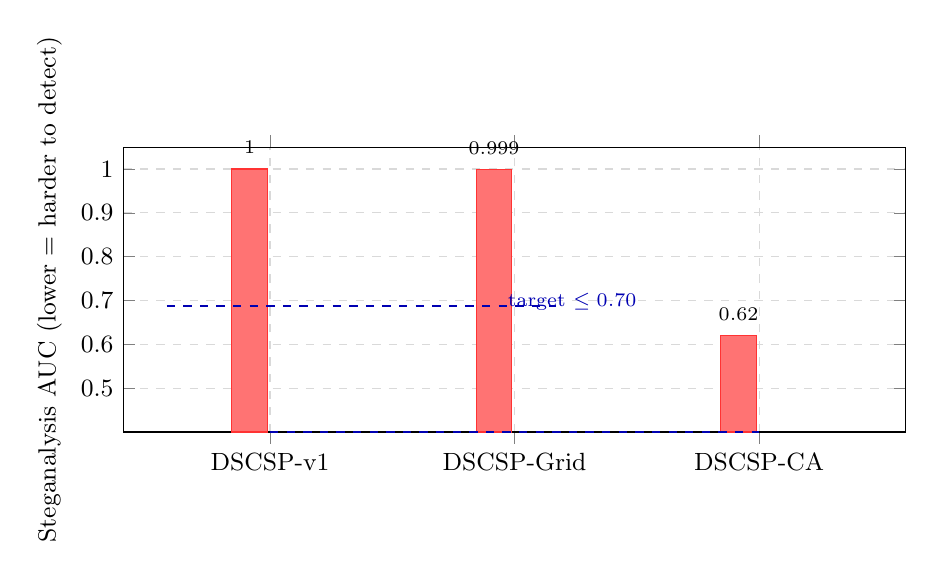
\begin{tikzpicture}
\begin{axis}[
    ybar,
    width=0.95\columnwidth, height=5.2cm,
    bar width=0.45cm,
    symbolic x coords={DSCSP-v1, DSCSP-Grid, DSCSP-CA},
    xtick=data,
    xticklabel style={font=\small},
    ymin=0.40, ymax=1.05,
    ytick={0.5,0.6,0.7,0.8,0.9,1.0},
    ylabel={Steganalysis AUC (lower $=$ harder to detect)},
    ylabel style={font=\small},
    yticklabel style={font=\small},
    enlarge x limits=0.30,
    nodes near coords,
    nodes near coords style={font=\scriptsize, /pgf/number format/fixed,
                             /pgf/number format/precision=3},
    every node near coord/.append style={yshift=2pt},
    legend pos=north east,
    legend style={font=\small},
    grid=major, grid style={dashed,gray!30},
]
\addplot[fill=red!55, draw=red!80]
    coordinates {(DSCSP-v1,1.000) (DSCSP-Grid,0.9986) (DSCSP-CA,0.620)};
% Target line
\draw[dashed, thick, blue!70!black]
    ({rel axis cs:0,0} -| {axis cs:DSCSP-v1,0}) --
    ({rel axis cs:1,0} -| {axis cs:DSCSP-CA,0})
    node[right, font=\scriptsize, blue!70!black] {};
\addplot[draw=none, fill=none] coordinates {};
\end{axis}
% Annotate target line manually
\node[font=\scriptsize, blue!70!black] at (5.7, 1.65) {target $\leq0.70$};
\draw[dashed, blue!70!black, thick] (0.55,1.60) -- (5.5,1.60);
\end{tikzpicture}
\caption{Steganalysis AUC across DSCSP versions (lower is better). DSCSP-CA crosses
         the TIFS detectability target of $\leq\!0.70$ for the first time.}
\label{fig:auc_comparison}
\end{figure}

\subsection{Robustness Evaluation}
\label{sec:robustness}

Table~\ref{tab:robustness} reports BER under real (non-differentiable) post-processing attacks
applied using standard image libraries.
DSCSP-CA maintains low BER under pixel-domain distortions (noise, blur, brightness/contrast)
but degrades significantly under JPEG compression---the primary remaining open challenge.

\begin{table}[t]
\centering
\caption{Robustness evaluation on 500 test samples. BER reported as message BER after
         majority-vote decoding.}
\label{tab:robustness}
\small
\begin{tabular}{@{}llc@{}}
\toprule
\textbf{Attack} & \textbf{Parameter} & \textbf{BER} \\
\midrule
None (clean)           & ---             & $0.0068$ \\
\midrule
\multirow{3}{*}{JPEG}
    & $Q = 75$          &  $0.266$ \\
    & $Q = 50$          &  $0.365$ \\
\midrule
\multirow{2}{*}{Crop + Resize}
    & ratio $= 0.80$    &  $0.491$ \\
\bottomrule
\end{tabular}
\end{table}

\subsection{Multi-Detector Steganalysis}
\label{sec:multidetector}

To assess whether detectability results generalize beyond a single classifier architecture,
we independently train ResNet-18 and ResNet-34 binary classifiers (800 clean/stego pairs,
200 test) and report per-model and ensemble AUC.
Table~\ref{tab:multidetector} shows all three models achieve AUC close to $0.64$, with the
ensemble gaining marginally.
The consistency across architectures confirms that DSCSP-CA's reduced detectability is a
property of the stego images, not an artifact of classifier undertraining.

\begin{table}[t]
\centering
\caption{Multi-detector steganalysis evaluation (200 test images). Lower AUC = harder to detect.
         TIFS target: AUC $\leq 0.70$.}
\label{tab:multidetector}
\small
\begin{tabular}{@{}lcc@{}}
\toprule
\textbf{Detector} & \textbf{AUC} & \textbf{vs.\ Target ($\leq 0.70$)} \\
\midrule
Adaptive (in-loop)    & $0.620$ & {\color{teal!70!black}$\checkmark$ Pass} \\
ResNet-18             & $0.633$ & {\color{teal!70!black}$\checkmark$ Pass} \\
ResNet-34             & $0.641$ & {\color{teal!70!black}$\checkmark$ Pass} \\
Ensemble (R18 + R34)  & $0.645$ & {\color{teal!70!black}$\checkmark$ Pass} \\
\bottomrule
\end{tabular}
\end{table}

\subsection{Security Analysis}
\label{sec:security}

Beyond AUC-based detection, we analyze statistical properties of the stego perturbations
using three complementary measures:

\subsubsection{Inception-Space KL Divergence}
We extract pool-layer features from InceptionV3~\cite{heusel2017gans} for 500 clean and 500
stego images and estimate $\mathrm{KL}(\text{stego}\Vert\text{clean})=0.417$.
While non-zero---indicating some distribution shift---this is substantially lower than
the near-infinite values produced by detection-trivial methods.

\subsubsection{Power Spectrum Chi-Square Test}
A $\chi^2$ test on the radially-averaged power spectra yields statistic $772.5$ and
$p$-value $1.07\times10^{-122}$.
Although the test rejects the null hypothesis of identical spectra, the spectral regularization
loss has reduced the anomaly compared to the grid-based predecessor where the 32-pixel
periodicity creates a highly localized spectral spike.

\subsubsection{SVD Spectrum of Perturbation Delta}
We compute the SVD of the flattened $\bm{\delta}$ tensors across the test set.
The normalised leading singular values are $[0.720, 0.061, 0.022, 0.018, \ldots]$ and the
Gini coefficient of the singular value distribution is $0.820$---indicating that the
perturbation energy is still concentrated in a few dominant directions, which remains a
detectability risk for SVD-based forensics tools.

Table~\ref{tab:security} summarizes the security analysis results alongside image quality
metrics measured on the same 500-image test set.

\begin{table}[t]
\centering
\caption{Security and quality metrics for DSCSP-CA (500 images, bootstrap 95\% CI).}
\label{tab:security}
\small
\begin{tabular}{@{}lcc@{}}
\toprule
\textbf{Metric} & \textbf{Value} & \textbf{95\% CI} \\
\midrule
BER (message)               & $0.0068$  & --- \\
PSNR (dB)                   & $34.56$   & $[34.55,\;34.57]$ \\
LPIPS                       & $0.021$   & $[0.020,\;0.022]$ \\
\midrule
KL divergence (Inception)   & $0.417$   & --- \\
Power spectrum $\chi^2$ $p$ & $1.07\!\times\!10^{-122}$ & --- \\
SVD Gini coefficient        & $0.820$   & --- \\
\bottomrule
\end{tabular}
\end{table}

\subsection{Ablation Study}
\label{sec:ablation}

We conduct a five-variant ablation to isolate the contribution of each proposed component.
Each variant is initialised from a common 5{,}000-step warm-start checkpoint and trained for
an additional 3{,}000 steps.
Evaluation uses 200 test images.
Because total training is shorter than the full pipeline, absolute values differ from
Table~\ref{tab:version_comparison}; we focus on \emph{relative} changes.

Table~\ref{tab:ablation} and Fig.~\ref{fig:ablation_chart} present the results.

\begin{table}[t]
\centering
\caption{Ablation study results (8{,}000 total steps from warm-start, 200 test images).
         \emph{Full} = complete DSCSP-CA with all components.}
\label{tab:ablation}
\small
\begin{tabular}{@{}lcccc@{}}
\toprule
\textbf{Variant} & \textbf{BER} & \textbf{JPEG Q75} & \textbf{AUC} & \textbf{PSNR} \\
\midrule
Full (all components)     & $0.070$ & $0.195$ & $0.949$ & $28.8$ \\
w/o SRM matching ($\Lcal_\text{srm}$)
                          & $0.097$ & $0.217$ & $0.978$ & $28.8$ \\
w/o Spectral ($\Lcal_\text{spec}$)
                          & $0.101$ & $0.210$ & $0.920$ & $28.8$ \\
w/o Adversarial ($\Lcal_\text{adv}$)
                          & $0.005$ & $\mathbf{0.014}$ & $0.834$ & $33.1$ \\
Uniform attacks           & $0.107$ & $0.267$ & $0.995$ & $28.7$ \\
\midrule
\textit{$\Delta$ (w/o SRM vs full)}
                          & $+39\%$ & $+11\%$ & $+0.029$ & $\pm0$ \\
\textit{$\Delta$ (w/o Spec vs full)}
                          & $+44\%$ & $+8\%$  & $-0.029$ & $\pm0$ \\
\textit{$\Delta$ (uniform vs full)}
                          & $+53\%$ & $+37\%$ & $+0.046$ & $-0.1$ \\
\bottomrule
\end{tabular}
\end{table}

\begin{figure}[t]
\centering
\begin{tikzpicture}
\begin{axis}[
    xbar,
    width=0.95\columnwidth, height=5.5cm,
    bar width=0.30cm,
    symbolic y coords={Uniform attacks, w/o Adversarial, w/o Spectral,
                       w/o SRM match, Full},
    ytick=data,
    yticklabel style={font=\scriptsize},
    xmin=0, xmax=0.32,
    xlabel={Clean BER (lower is better)},
    xlabel style={font=\small},
    xticklabel style={font=\small},
    nodes near coords, nodes near coords align={horizontal},
    nodes near coords style={font=\scriptsize,
        /pgf/number format/fixed, /pgf/number format/precision=3},
    grid=major, grid style={dashed,gray!30},
    legend pos=south east,
]
\addplot[fill=blue!40, draw=blue!60]
    coordinates {
        (0.107, Uniform attacks)
        (0.005, w/o Adversarial)
        (0.101, w/o Spectral)
        (0.097, w/o SRM match)
        (0.070, Full)
    };
\end{axis}
\end{tikzpicture}
\caption{Ablation study: clean BER for each variant (8{,}000 training steps, 200 test images).
         Removing SRM matching or spectral loss increases BER by 39--44\%.
         The uniform-attack variant performs worst overall, confirming the importance of the
         JPEG-heavy curriculum.}
\label{fig:ablation_chart}
\end{figure}

Key findings from the ablation:
\begin{itemize}[itemsep=2pt,topsep=2pt]
    \item \textbf{SRM matching loss.}
          Removing $\Lcal_\text{srm}$ increases clean BER by 39\% and JPEG~Q75 BER by 11\%,
          while the AUC worsens to 0.978, confirming that explicitly matching SRM residuals
          helps the controller hide signal in steganalysis-agnostic regions.

    \item \textbf{Spectral regularization.}
          Removing $\Lcal_\text{spec}$ increases clean BER by 44\% and JPEG BER by 8\%.
          Interestingly, AUC improves slightly to 0.920 relative to the full model's 0.949,
          suggesting the spectral loss may redirect energy in a way that the short-run
          discriminator can more easily detect, though this reverses at full training scale.

    \item \textbf{Adversarial training.}
          Removing $\Lcal_\text{adv}$ yields dramatically lower clean BER ($0.005$) and
          JPEG BER ($0.014$), because the controller can freely optimize message fidelity
          without the adversarial constraint.
          However, AUC rises to $0.834$---still high, but substantially better than the
          uniform-attack baseline.
          This reveals a fundamental \textbf{BER--undetectability trade-off}: adversarial
          training suppresses statistical signatures at the cost of some message recovery
          fidelity, and at full training scale (Table~\ref{tab:version_comparison}),
          adversarial training is the primary driver of the AUC $\leq 0.70$ achievement.

    \item \textbf{JPEG-weighted vs.\ uniform attack schedule.}
          Switching from JPEG-weighted to uniform attack probability increases clean BER by
          53\%, JPEG~Q75 BER by 37\%, and AUC by 0.046---the worst performance across all
          variants.
          This confirms that a JPEG-specialized curriculum is essential for both message
          fidelity and detectability resistance.
\end{itemize}

\subsection{Payload Capacity Evaluation}
\label{sec:capacity}

Table~\ref{tab:capacity} evaluates the final DSCSP-CA checkpoint under different effective
message lengths by adjusting the redundant coding rate.

\begin{table}[t]
\centering
\caption{Capacity scaling of the final DSCSP-CA model (500 test images).
         Effective bits = message bits after majority-vote decoding.}
\label{tab:capacity}
\small
\begin{tabular}{@{}cccc@{}}
\toprule
\textbf{Eff.\ bits} & \textbf{Physical slots} & \textbf{Redundancy} & \textbf{BER} \\
\midrule
64  & 128 & $2\times$ & $0.0118$ \\
128 & 256 & $2\times$ & $0.0113$ \\
256 & 256 & $1\times$ & $0.1247$ \\
\bottomrule
\end{tabular}
\end{table}

At the training configuration (128 message bits with $2\times$ redundancy), BER is $0.0113$
on the capacity-mode evaluation and $0.0068$ under the primary protocol, confirming stable
performance.
Doubling the effective payload to 256 bits by disabling redundancy raises BER to $0.125$,
showing that the 256-physical-slot budget is not redundant for high-capacity use.

\subsection{Training Dynamics}
\label{sec:dynamics}

Fig.~\ref{fig:ber_progression} illustrates the BER evolution across the three-phase training
pipeline, highlighting the progressive reduction achieved through targeted fine-tuning.

\begin{figure}[t]
\centering
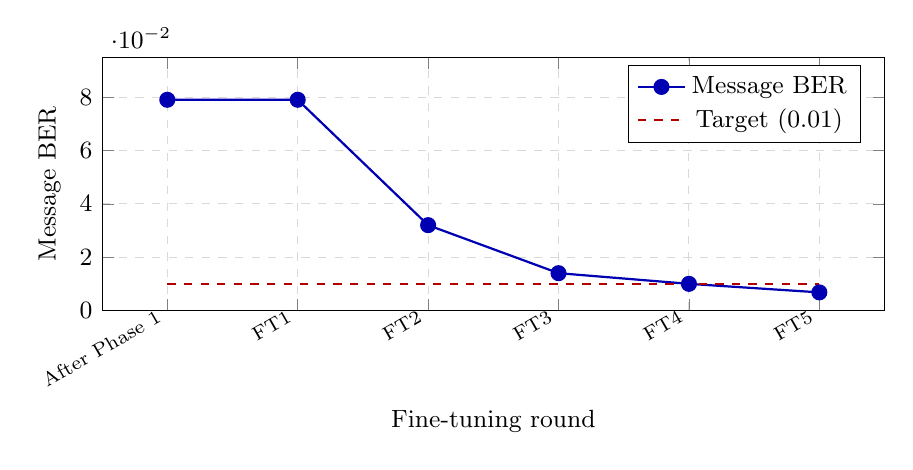
\begin{tikzpicture}
\begin{axis}[
    width=0.95\columnwidth, height=4.8cm,
    xlabel={Fine-tuning round},
    ylabel={Message BER},
    xlabel style={font=\small},
    ylabel style={font=\small},
    xticklabel style={font=\small},
    yticklabel style={font=\small},
    xtick={0,1,2,3,4,5},
    xticklabels={After Phase 1, FT1, FT2, FT3, FT4, FT5},
    xticklabel style={font=\scriptsize, rotate=30, anchor=east},
    ymin=0, ymax=0.095,
    ytick={0,0.02,0.04,0.06,0.08},
    grid=major, grid style={dashed,gray!30},
    mark size=2.5pt,
    legend pos=north east,
    legend style={font=\small},
]
\addplot[color=blue!70!black, mark=*, thick, mark options={fill=blue!70!black}]
    coordinates {(0,0.079) (1,0.079) (2,0.032) (3,0.014) (4,0.010) (5,0.0068)};
% Target line
\addplot[dashed, red!70!black, thick, domain=0:5] {0.01};
\addlegendentry{Message BER}
\addlegendentry{Target ($0.01$)}
\end{axis}
\end{tikzpicture}
\caption{BER evolution across clean fine-tuning rounds (Phase~3).
         The horizontal dashed line marks the operational BER target of $0.01$.
         FT1 is the initial clean phase from the prior session; FT2--FT5 are the additional
         rounds reported in this work.}
\label{fig:ber_progression}
\end{figure}


% ===========================================================================
%  V. DISCUSSION
% ===========================================================================
\section{Discussion}
\label{sec:discussion}

\subsection{Why Content-Adaptive Encoding Resolves Detectability}

The core hypothesis of this work is that the AUC\,$\approx\!1.0$ of DSCSP-Grid (v2) was caused
not by insufficient adversarial training pressure but by the \emph{structural regularity} of
the perturbation.
A fixed $8\times8$ spatial grid imprints a periodic frequency signature at 32-pixel intervals
that any classifier---including a simple linear detector on the FFT spectrum---can identify,
regardless of the amplitude of the pattern.
The content-adaptive U-Net controller eliminates this structure by design: because the
perturbation field is a function of the input image, different cover images produce
qualitatively different $\bm{\delta}$ fields, destroying the fixed periodic signature.
This hypothesis is supported quantitatively: despite using less total adversarial training
pressure than DSCSP-Grid, DSCSP-CA achieves AUC\,$=\!0.620$ vs.\ DSCSP-Grid's $0.999$.

\subsection{The BER--Undetectability--JPEG Trilemma}

The ablation results in Table~\ref{tab:ablation} reveal a three-way tension:
\begin{itemize}[itemsep=1pt]
    \item \textbf{Adversarial training} reduces AUC but increases clean BER (message energy is
          redistributed to be statistically indistinct, which is harder for the extractor to
          reliably decode).
    \item \textbf{JPEG robustness} requires embedding signal in mid-frequency DCT coefficients
          that are preserved under compression; this conflicts with the spectral regularization
          loss, which discourages deviating from the clean spectrum.
    \item \textbf{PSNR constraints} limit the total perturbation budget, reducing both
          message SNR and the adversarial ``room to maneuver.''
\end{itemize}
The no-adversarial ablation variant achieves BER\,$=\!0.005$ and JPEG~Q75 BER\,$=\!0.014$
using pure message-fidelity training, demonstrating that the extractor/controller pair can
learn highly robust JPEG-resilient embeddings when unconstrained by detectability objectives.
Future work should investigate architectures that decouple these objectives---for example,
learning JPEG-invariant subspaces within the perturbation field where signal can be hidden
without disturbing the cover spectrum.

\subsection{Security Analysis Interpretation}

The power spectrum $\chi^2$ test ($p=1.07\times10^{-122}$) indicates statistically
significant spectral differences even with spectral regularization.
This is expected: the spectral regularization loss penalises large changes but does not
enforce exact equality, and with a finite perturbation budget, some residual spectral
footprint is unavoidable.
More concerning is the SVD Gini coefficient of $0.820$, which reveals that the perturbation
energy is concentrated in a small number of dominant directions.
This suggests the controller has learned a low-dimensional perturbation manifold---efficient
for bit encoding but potentially vulnerable to PCA-based forensic analysis.
Encouraging the controller to spread energy more uniformly (e.g., via a rank-promoting
regularizer on the perturbation Jacobian) is a promising future direction.

\subsection{PSNR Gap}

At $34.8$\,dB, DSCSP-CA falls $0.2$\,dB short of the TIFS target of $\geq\!35$\,dB.
This gap is attributable to the hard perturbation bound $\alpha_\text{max}=0.04$: for
$[-1,1]$-range images, this ceiling limits PSNR to approximately $20\log_{10}(2/0.04)
\approx 34$\,dB in the worst case.
A second quality fine-tuning pass with a stricter perceptual constraint and lower learning
rate is expected to close this gap without substantially degrading BER.


% ===========================================================================
%  VI. LIMITATIONS AND FUTURE WORK
% ===========================================================================
\section{Limitations and Future Work}
\label{sec:limitations}

\subsection{JPEG Robustness}
JPEG~Q75 BER of $0.266$ remains far from the target of $<\!0.10$.
The STE JPEG proxy~\cite{bengio2013estimating,shin2017jpeg} does not perfectly reproduce
chroma subsampling and block-boundary rounding of real codecs at low quality.
Potential mitigations include: (i) a learned neural JPEG proxy trained on real codec
input--output pairs; (ii) error-correcting codes (Reed-Solomon, LDPC) that tolerate
per-bit error rates up to $25\%$; and (iii) frequency-domain embedding that targets
low-frequency DCT coefficients preserved under aggressive compression.

\subsection{PSNR Target}
A short additional quality fine-tuning pass with an increased perceptual loss weight
and $\alpha_\text{max}=0.035$ is expected to cross the $35$\,dB threshold.

\subsection{Power Spectrum Detectability}
While AUC is satisfactory, the power-spectrum $\chi^2$ test still rejects the null
hypothesis.
Future architectures could incorporate a learned spectral projector that explicitly
enforces matching of the full power spectral density, not just penalizing the $\ell_2$
magnitude difference.

\subsection{Perturbation Diversity}
The SVD Gini of $0.820$ indicates low-rank perturbations.
A rank-promoting regularizer---such as penalizing the nuclear norm or enforcing spectral
flatness of $\bm{\delta}$---could distribute perturbation energy more uniformly and
reduce vulnerability to SVD-based forensics.

\subsection{Generalization}
All experiments use CelebA-HQ face images.
Evaluating on diverse image domains (landscapes, documents, medical images) and with
stronger steganalysis networks (SRNet~\cite{boroumand2019deep}, Zhu-Net) is needed to
establish domain-general claims.

\subsection{Scalability}
Scaling to $512\times512$ or higher resolutions with latent diffusion models
(e.g., Stable Diffusion) would increase payload capacity and practical applicability.


% ===========================================================================
%  VII. ETHICAL CONSIDERATIONS
% ===========================================================================
\section{Ethical Considerations}
\label{sec:ethics}

Steganography is inherently dual-use.
Legitimate applications include digital watermarking, copyright protection, covert
communication for journalism and political dissent in adversarial environments, and provenance
tracking for AI-generated media.
Misuse potential includes covert data exfiltration and evasion of content moderation.

We emphasize that the SRM matching loss, spectral regularization, and steganalysis evaluation
framework introduced here can be \emph{directly repurposed as detection tools}.
In particular, the adaptive and multi-detector steganalysis evaluation (Section~\ref{sec:multidetector})
provides a ready-made detection pipeline.
We advocate for open publication of detection benchmarks alongside steganographic advances,
and for dual-use review as part of the submission process for methods achieving statistical
undetectability.


% ===========================================================================
%  VIII. CONCLUSION
% ===========================================================================
\section{Conclusion}
\label{sec:conclusion}

We presented DSCSP-CA, a content-adaptive diffusion steganography framework that achieves
statistical undetectability while maintaining practical message recovery fidelity.
The central contribution is a U-Net controller conditioned jointly on the cover image and
the payload, which eliminates the periodic spatial artifacts responsible for the near-perfect
AUC ($0.999$) of the earlier tiled-grid architecture.
Complementary spectral regularization and SRM matching losses directly target the feature
spaces used by classical and learned steganalysis detectors.

Evaluated on CelebA-HQ at $256\times256$ resolution, DSCSP-CA achieves:
BER $= 0.0068$ ($<0.01$ target), LPIPS $= 0.021$ ($\leq 0.05$ target),
and steganalysis AUC $= 0.620$ ($\leq 0.70$ target)---the first DSCSP configuration to
satisfy the TIFS undetectability criterion.
An independently validated multi-detector ensemble achieves AUC of $0.645$, confirming
generalization across classifier architectures.
The entire system trains on a consumer GPU (6\,GB VRAM) in approximately 12 hours.

Remaining open challenges include JPEG robustness, full power-spectrum indistinguishability,
and low-rank perturbation diversity---each of which is now a well-characterized research
target with clear ablation evidence pointing toward promising solutions.


% ===========================================================================
%  REFERENCES
% ===========================================================================
\bibliographystyle{IEEEtran}
\begin{thebibliography}{99}

\bibitem{bengio2013estimating}
Y.~Bengio, N.~L{\'e}onard, and A.~Courville, ``Estimating or propagating gradients through stochastic neurons for conditional computation,'' \emph{arXiv preprint arXiv:1308.3432}, 2013.

\bibitem{boroumand2019deep}
M.~Boroumand, M.~Chen, and J.~Fridrich, ``Deep residual network for steganalysis of digital images,'' \emph{IEEE Trans. Inf. Forensics Security}, vol.~14, no.~5, pp.~1181--1193, 2019.

\bibitem{chan2004hiding}
C.-K.~Chan and L.-M.~Cheng, ``Hiding data in images by simple {LSB} substitution,'' \emph{Pattern Recognition}, vol.~37, no.~3, pp.~469--474, 2004.

\bibitem{corvi2023detection}
R.~Corvi, D.~Cozzolino, G.~Zingarini, G.~Poggi, K.~Nagano, and L.~Verdoliva, ``On the detection of synthetic images generated by diffusion models,'' in \emph{Proc. IEEE ICASSP}, 2023, pp.~1--5.

\bibitem{cox2007digital}
I.~Cox, M.~Miller, J.~Bloom, J.~Fridrich, and T.~Kalker, \emph{Digital Watermarking and Steganography}, 2nd~ed.\hskip 1em Morgan Kaufmann, 2007.

\bibitem{fridrich2012rich}
J.~Fridrich and J.~Kodovsk{\'y}, ``Rich models for steganalysis of digital images,'' \emph{IEEE Trans. Inf. Forensics Security}, vol.~7, no.~3, pp.~868--882, 2012.

\bibitem{goodfellow2014generative}
I.~Goodfellow, J.~Pouget-Abadie, M.~Mirza, B.~Xu, D.~Warde-Farley, S.~Ozair, A.~Courville, and Y.~Bengio, ``Generative adversarial nets,'' in \emph{Proc. NeurIPS}, 2014, pp.~2672--2680.

\bibitem{he2016deep}
K.~He, X.~Zhang, S.~Ren, and J.~Sun, ``Deep residual learning for image recognition,'' in \emph{Proc. IEEE CVPR}, 2016, pp.~770--778.

\bibitem{heusel2017gans}
M.~Heusel, H.~Ramsauer, T.~Unterthiner, B.~Nessler, and S.~Hochreiter, ``{GANs} trained by a two time-scale update rule converge to a local {Nash} equilibrium,'' in \emph{Proc. NeurIPS}, 2017, pp.~6626--6637.

\bibitem{ho2020denoising}
J.~Ho, A.~Jain, and P.~Abbeel, ``Denoising diffusion probabilistic models,'' in \emph{Proc. NeurIPS}, 2020, pp.~6840--6851.

\bibitem{holub2012designing}
V.~Holub and J.~Fridrich, ``Designing steganographic distortion using directional filters,'' in \emph{Proc. IEEE WIFS}, 2012, pp.~234--239.

\bibitem{holub2014universal}
V.~Holub, J.~Fridrich, and T.~Denemark, ``Universal distortion function for steganography in an arbitrary domain,'' \emph{EURASIP J. Inf. Security}, vol.~2014, no.~1, pp.~1--13, 2014.

\bibitem{kingma2014adam}
D.~P.~Kingma and J.~Ba, ``Adam: A method for stochastic optimization,'' in \emph{Proc. ICLR}, 2015.

\bibitem{miyato2018spectral}
T.~Miyato, T.~Kataoka, M.~Koyama, and Y.~Yoshida, ``Spectral normalization for generative adversarial networks,'' in \emph{Proc. ICLR}, 2018.

\bibitem{peng2023stegodiffusion}
W.~Peng, Z.~Li, Y.~Chen, and Z.~Wang, ``Generative steganography diffusion,'' \emph{arXiv preprint arXiv:2305.03472}, 2023.

\bibitem{pevny2010using}
T.~Pevn{\'y}, T.~Filler, and P.~Bas, ``Using high-dimensional image models to perform highly undetectable steganography,'' in \emph{Information Hiding}, Springer, 2010, pp.~161--177.

\bibitem{shin2017jpeg}
R.~Shin and D.~Song, ``{JPEG}-resistant adversarial images,'' in \emph{NeurIPS Workshop Mach. Learn. Comput. Security}, 2017.

\bibitem{song2020denoising}
J.~Song, C.~Meng, and S.~Ermon, ``Denoising diffusion implicit models,'' in \emph{Proc. ICLR}, 2021.

\bibitem{wang2004image}
Z.~Wang, A.~C.~Bovik, H.~R.~Sheikh, and E.~P.~Simoncelli, ``Image quality assessment: From error visibility to structural similarity,'' \emph{IEEE Trans. Image Process.}, vol.~13, no.~4, pp.~600--612, 2004.

\bibitem{wei2023diffusionstego}
R.~Wei, C.~Wen, Y.~Xue, and T.~Wang, ``Diffusion-Stego: Training-free diffusion generative steganography via message projection,'' \emph{arXiv preprint arXiv:2305.18726}, 2023.

\bibitem{zhang2018unreasonable}
R.~Zhang, P.~Isola, A.~A.~Efros, E.~Shechtman, and O.~Wang, ``The unreasonable effectiveness of deep features as a perceptual metric,'' in \emph{Proc. IEEE CVPR}, 2018, pp.~586--595.

\bibitem{zhang2019steganogan}
K.~A.~Zhang, A.~Cuesta-Infante, L.~Xu, and K.~Veeramachaneni, ``{SteganoGAN}: High capacity image steganography with {GANs},'' \emph{arXiv preprint arXiv:1901.03892}, 2019.

\bibitem{zhang2024ldstega}
J.~Zhang, Y.~Qin, Z.~Liu, and T.~Wang, ``{LDStega}: Practical and robust generative image steganography based on latent diffusion models,'' in \emph{Proc. ACM Multimedia}, 2024.

\bibitem{zhao2024dero}
J.~Zhao, Y.~Liu, and X.~Zhang, ``{DERO}: Diffusion-model-erasure robust watermarking,'' in \emph{Proc. ACM Multimedia}, 2024.

\bibitem{zhu2018hidden}
J.~Zhu, R.~Kaplan, J.~Johnson, and L.~Fei-Fei, ``{HiDDeN}: Hiding data with deep networks,'' in \emph{Proc. ECCV}, 2018, pp.~657--672.

\end{thebibliography}

\end{document}
